\documentclass{beamer}

\usepackage[utf8]{inputenc}
\usecolortheme{beaver}
\usepackage{caption}
\usepackage{subcaption}
\usepackage{mathtools}
\usepackage{todonotes}
\usepackage{amsmath}
\usepackage{bm}
\usepackage{listings}
\usepackage{ragged2e}
\usepackage{titlecaps}
\usepackage{fancyvrb}

\def\ci{\perp\!\!\!\!\!\perp}

\newtheorem{proposition}{Proposition}
\Addlcwords{for a is but and with of in as the etc on to if}

\setbeamertemplate{section in toc}{\inserttocsectionnumber.~\inserttocsection}
\usetheme{Boadilla}
\makeatletter
\setbeamertemplate{footline}{%
    \leavevmode%
    \hbox{%
        \begin{beamercolorbox}[wd=.3\paperwidth,ht=2.25ex,dp=1ex,center]{author in head/foot}%
            \usebeamerfont{author in head/foot}\insertshortauthor\expandafter\beamer@ifempty\expandafter{\beamer@shortinstitute}{}{~~(\insertshortinstitute)}
        \end{beamercolorbox}%
        \begin{beamercolorbox}[wd=.55\paperwidth,ht=2.25ex,dp=1ex,center]{title in head/foot}%
            \usebeamerfont{title in head/foot}\insertshorttitle
        \end{beamercolorbox}%
        \begin{beamercolorbox}[wd=.15\paperwidth,ht=2.25ex,dp=1ex,right]{date in head/foot}%
            \usebeamerfont{date in head/foot}\insertshortdate{}\hspace*{2em}
            \insertframenumber{} / \inserttotalframenumber\hspace*{2ex} 
        \end{beamercolorbox}}%
        \vskip0pt%
    }
\makeatother

\begin{document}

\title[]{Expert-in-the-Loop Causal Discovery}
\author{Ankur Ankan}
\date{}

\maketitle

\begin{frame}{Directed Acyclic Graphs (DAGs)}
	\begin{columns}
		\begin{column}{0.6 \textwidth}
		\begin{itemize}
			\item Nodes represent random variables.
			\item Edges represent causal relationships.
			\item E.g., \textbf{Education} has a direct effect on \textbf{Income}. 
			\item \textbf{Age} has indirect effect on \textbf{Income} through \textbf{Education} and \textbf{Hours Per Week}.
			\item Used for causal effect estimation.
		\end{itemize}
		\end{column}

		\begin{column}{0.45 \textwidth}
		\begin{figure}
			\centering
			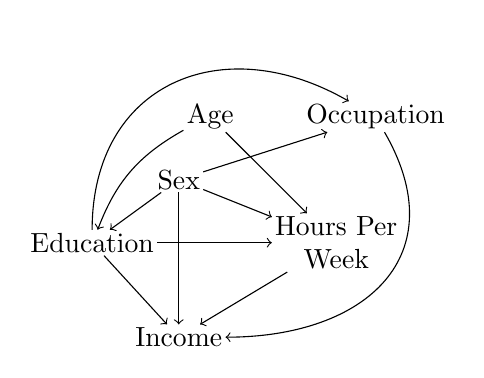
\begin{tikzpicture}[scale=1]
			\tikzstyle{every node}=[align=center, inner sep=1pt]
				\node (sex) at (-0.7, -0.8) {Sex};
				\node (age) at (-0.3, 0) {Age};
				\node (ed) at (-1.8, -1.6) {Education};
				\node (occ) at (1.8, 0) {Occupation};
				\node (hrpw) at (1.3, -1.6) {Hours Per \\ Week};
				\node (income) at (-0.7, -2.8) {Income};
			
				\draw[->]  (age) to[bend right=20] (ed);
				\draw[->]  (sex) to (ed);
				\draw[->]  (age) to (hrpw);
				\draw[->]  (ed) to (hrpw);
				\draw[->]  (sex) to (hrpw);
				\draw[->]  (ed) to (income);
				\draw[->]  (hrpw) to (income);
				\draw[->]  (occ) to[out=300, in=0, looseness=1.4] (income.east);
				\draw[->]  (sex) to (income);
				\draw[->]  (ed) to[out=90, in=150, looseness=1.3] (occ);
				\draw[->]  (sex) to (occ);	
			\end{tikzpicture}
			\caption{Example of a DAG}
		\end{figure}
		\end{column}
	\end{columns}	
\end{frame}

\begin{frame}{Causal Discovery: Learning DAGs From Data}
	\vspace{-2em}
	\begin{figure}
		\centering
		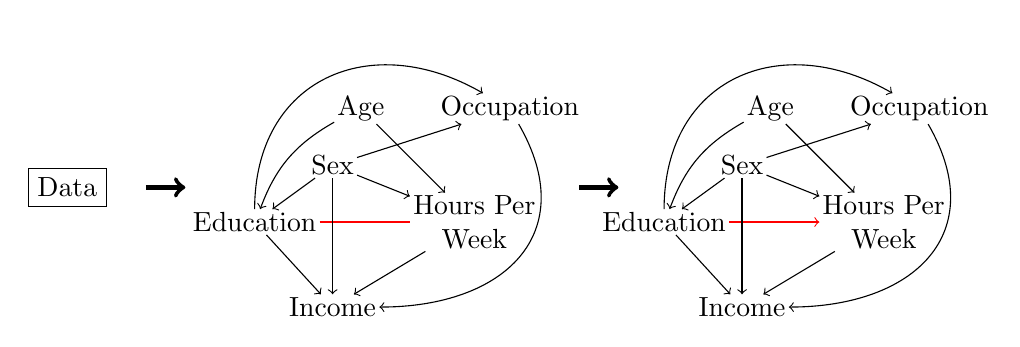
\begin{tikzpicture}
			\node[draw, rectangle] (data) at (0, 0) {Data};
			\draw[ultra thick,->] (1,0) -- (1.5,0);
			\begin{scope}[xshift=4cm, yshift=1cm, scale=0.9]
			 	\tikzstyle{every node}=[align=center, inner sep=1pt]
				\node (sex) at (-0.7, -0.8) {Sex};
				\node (age) at (-0.3, 0) {Age};
				\node (ed) at (-1.8, -1.6) {Education};
				\node (occ) at (1.8, 0) {Occupation};
				\node (hrpw) at (1.3, -1.6) {Hours Per \\ Week};
				\node (income) at (-0.7, -2.8) {Income};
			
				\draw[->]  (age) to[bend right=20] (ed);
				\draw[->]  (sex) to (ed);
				\draw[->]  (age) to (hrpw);
				\draw[-, red]  (ed) to (hrpw);
				\draw[->]  (sex) to (hrpw);
				\draw[->]  (ed) to (income);
				\draw[->]  (hrpw) to (income);
				\draw[->]  (occ) to[out=300, in=0, looseness=1.4] (income.east);
				\draw[->]  (sex) to (income);
				\draw[->]  (ed) to[out=90, in=150, looseness=1.3] (occ);
				\draw[->]  (sex) to (occ);	
			\end{scope}
			\begin{scope}[xshift=6.5cm]
				\draw[ultra thick,->] (0,0) -- (0.5,0);
			\end{scope}	
			\begin{scope}[xshift=9.2cm, yshift=1cm, scale=0.9]
				\tikzstyle{every node}=[align=center, inner sep=1pt]
				\node (sex) at (-0.7, -0.8) {Sex};
				\node (age) at (-0.3, 0) {Age};
				\node (ed) at (-1.8, -1.6) {Education};
				\node (occ) at (1.8, 0) {Occupation};
				\node (hrpw) at (1.3, -1.6) {Hours Per \\ Week};
				\node (income) at (-0.7, -2.8) {Income};
			
				\draw[->]  (age) to[bend right=20] (ed);
				\draw[->]  (sex) to (ed);
				\draw[->]  (age) to (hrpw);
				\draw[->, red]  (ed) to (hrpw);
				\draw[->]  (sex) to (hrpw);
				\draw[->]  (ed) to (income);
				\draw[->]  (hrpw) to (income);
				\draw[->]  (occ) to[out=300, in=0, looseness=1.4] (income.east);
				\draw[->]  (sex) to (income);
				\draw[->]  (ed) to[out=90, in=150, looseness=1.3] (occ);
				\draw[->]  (sex) to (occ);	
			\end{scope}
		\end{tikzpicture}
	\end{figure}

	\begin{itemize}
		\item Causal Discovery: Recover DAG from data.
		\item Many algorithms are available:
			\begin{itemize}
				\item Constraint Based: PC, FCI
				\item Score Based: Hill-Climb Search, GES
				\item Optimization Based: No Tears
			\end{itemize}
		\item Algorithms can only recover Markov Equivalence Class i.e. CPDAG.
		\item Either expert knowledge or some further assumptions can
			be make to orient the edges.
	\end{itemize}
\end{frame}

\begin{frame}{Causal Discovery in Practice}
	\begin{itemize}
		\item Adaption of causal discovery algorithms is very limited.
		\item Researchers prefer to draw models by hand based on domain knowledge.
		\item Potential reasons could be:
			\begin{itemize}
				\item Algorithms can make obvious mistakes, making it harder to trust.
				\item Hard to choose an algorithm for a given dataset because of the different assumptions.
				\item No way to evaluate algorithm performance on a given dataset.
			\end{itemize}
		\item However, some researchers do test their model against data.
	\end{itemize}
\end{frame}

\begin{frame}{Model Testing}
	\begin{figure}
		\centering
		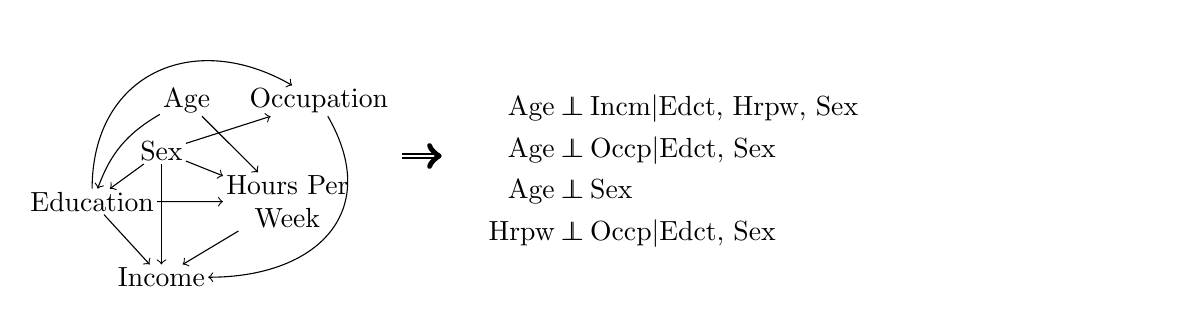
\begin{tikzpicture}
			\begin{scope}[yshift=0.7cm, scale=0.8]
			\tikzstyle{every node}=[align=center, inner sep=1pt]
				\node (sex) at (-0.7, -0.8) {Sex};
				\node (age) at (-0.3, 0) {Age};
				\node (ed) at (-1.8, -1.6) {Education};
				\node (occ) at (1.8, 0) {Occupation};
				\node (hrpw) at (1.3, -1.6) {Hours Per \\ Week};
				\node (income) at (-0.7, -2.8) {Income};
			
				\draw[->]  (age) to[bend right=20] (ed);
				\draw[->]  (sex) to (ed);
				\draw[->]  (age) to (hrpw);
				\draw[->]  (ed) to (hrpw);
				\draw[->]  (sex) to (hrpw);
				\draw[->]  (ed) to (income);
				\draw[->]  (hrpw) to (income);
				\draw[->]  (occ) to[out=300, in=0, looseness=1.4] (income.east);
				\draw[->]  (sex) to (income);
				\draw[->]  (ed) to[out=90, in=150, looseness=1.3] (occ);
				\draw[->]  (sex) to (occ);	
			\end{scope}
			\draw[thick, ->, double] (2.5,0) -- (3,0);
			\node[rectangle, align=center, inner sep=1pt] at (6, 0) {
				\begin{minipage}{\textwidth}
					\begin{equation*}
						\begin{split}
							\textnormal{Age} &\ci \textnormal{Incm} \rvert \textnormal{Edct, Hrpw, Sex} \\
							\textnormal{Age} &\ci \textnormal{Occp} \rvert \textnormal{Edct, Sex} \\
							\textnormal{Age} &\ci \textnormal{Sex} \\
							\textnormal{Hrpw} &\ci \textnormal{Occp} \rvert \textnormal{Edct, Sex} \\
						\end{split}
					\end{equation*}
				\end{minipage}
				};
		\end{tikzpicture}
	\end{figure}

	\vspace{2em}
	\begin{itemize}
		\item Each missing edge implies a Conditional Independence (CI).
		\item Statistical tests can be used to check whether they hold in data.
	\end{itemize}
\end{frame}

\begin{frame}{CI Tests and Effect Sizes}
	We can also use CI tests to estimate effect sizes of edges.
	\begin{figure}
		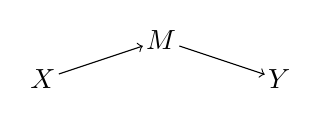
\begin{tikzpicture}[scale=1]
			\tikzstyle{every node}=[align=center, inner sep=1pt]
				\node (X) at (0, 0) {$ X $};
				\node (M) at (1.5, 0.5) {$ M $};
				\node (Y) at (3, 0) {$ Y $};
				\draw[->]  (X) to (M);
				\draw[->]  (M) to (Y);
		\end{tikzpicture}
	\end{figure}
\end{frame}

\begin{frame}{Deciding edges between variables based on effect sizes}
	The CI tests gives an effect size that can be used to decide whether an edge exists or not.
	
	The direction of these edges are still unknown, the expert needs to specify the
	direction.

	\todo[inline]{Show an example of the mediator model here to explain how can we decide}
\end{frame}

\begin{frame}{Human-in-the-loop Structure Learning}
	\begin{itemize}
		\item Based on this CI testing, we built a web-based tool to assist in constructing DAGs.
		\item Given a dataset, the tool shows all unexplained correlations between variables.
		\item It also shows when certain edges do not add any extra explanation between variables.
	\end{itemize}
\end{frame}

\begin{frame}
	\center \huge DEMO
\end{frame}

\begin{frame}{Effect Sizes}
	Marginal: Just the correlation between the variables.
	Conditional: Partial correlation
	Given $ X \ci Y | Z $
	\begin{itemize}
		\item Train estimators $ f_X: X \sim Z $ and $ f_Y: Y \sim Z $.
		\item Take residuals from the estimators: $ R_X = X - f_X(Z) $ and $ R_Y = Y - f_Y(Z) $.
		\item $ \rho = cor(R_X, R_Y) $.
	\end{itemize}

	For discrete variables Cramer's V can be used.
\end{frame}

\begin{frame}{Effect Sizes}
	However, there are no effect sizes for mixed data. We propose one based on
	canonical correlations.

	1. Marginal Case: Take the canonical correlation between normal or dummy encoded variables.

	2. Conditional Case: Use a similar approach as partial correlation, build two 
		estimators, use a residualization approach from previous paper, take
		the canonical correlation based effect size between them.


\end{frame}

\begin{frame}

	Canonical Correlations have some nice properties: 1) Reduces down to know effect size measures in standard cases. 2) Bounded between $ 0 $ and $ 1 $.

\end{frame}

\begin{frame}{Empirical Analysis: Simulate Expert}

	\begin{figure}
		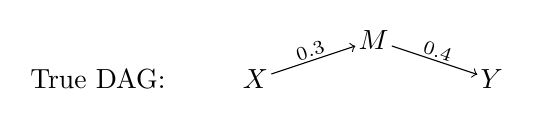
\begin{tikzpicture}[scale=1]
			\tikzstyle{every node}=[align=center, inner sep=1pt]
				\node (text) at (-2, 0) {True DAG:};
				\node (X) at (0, 0) {$ X $};
				\node (M) at (1.5, 0.5) {$ M $};
				\node (Y) at (3, 0) {$ Y $};
				\draw[->]  (X) -- node[midway, sloped, above] {\scriptsize $ 0.3 $} (M);
				\draw[->]  (M) -- node[midway, sloped, above] {\scriptsize $ 0.4 $} (Y);
		\end{tikzpicture}
	\end{figure}
	
	\vspace{2em}

	\begin{figure}
		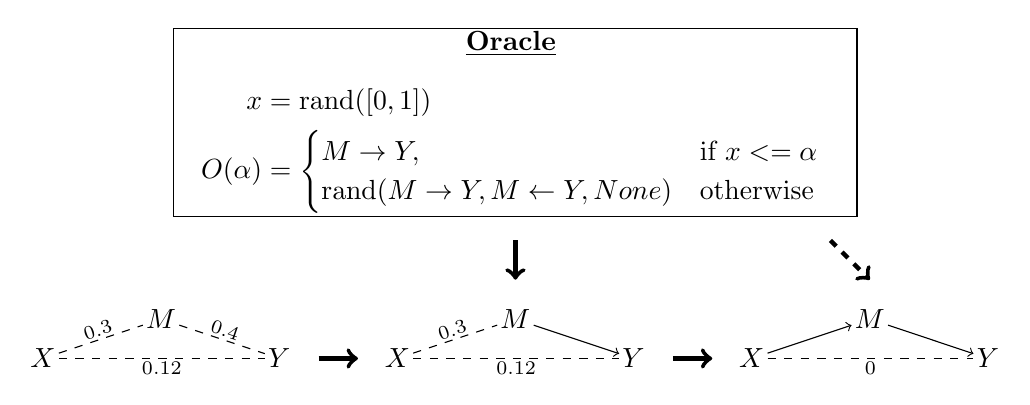
\begin{tikzpicture}
				\begin{scope}
					\tikzstyle{every node}=[align=center, inner sep=1pt]
					\node (X) at (0, 0) {$ X $};
					\node (M) at (1.5, 0.5) {$ M $};
					\node (Y) at (3, 0) {$ Y $};
					\draw[dashed]  (X) -- node[midway, sloped, above] {\scriptsize $ 0.3 $} (M);
					\draw[dashed]  (M) -- node[midway, sloped, above] {\scriptsize $ 0.4 $} (Y);
					\draw[dashed]  (X) -- node[midway, sloped, below] {\scriptsize $ 0.12 $} (Y);
				\end{scope}
				\begin{scope}[xshift=3cm]
					\draw[->, ultra thick] (0.5, 0) -- (1, 0);
				\end{scope}
				\begin{scope}[xshift=6cm, yshift=3cm]
					\node[rectangle, draw, align=center, inner sep=1pt] at (0, 0) {
							\begin{minipage}{0.7\textwidth}
								\center{\underline{\textbf{Oracle}}}
								\begin{equation*}
								\begin{split}
									x &= \textnormal{rand}([0, 1]) \\
									O(\alpha) &= \begin{cases} 
										M \rightarrow Y, & \textnormal{if  } x <= \alpha \\
										\textnormal{rand}(M \rightarrow Y, M \leftarrow Y, None) & \textnormal{otherwise} \\
										     \end{cases} \\
								\end{split}
								\end{equation*}
							\end{minipage}
					};
				\end{scope}
				\begin{scope}[xshift=6cm, yshift=1cm]
					\draw[->, ultra thick] (0, 0.5) -- (0, 0);
				\end{scope}
				\begin{scope}[xshift=4.5cm]
					\tikzstyle{every node}=[align=center, inner sep=1pt]
					\node (X) at (0, 0) {$ X $};
					\node (M) at (1.5, 0.5) {$ M $};
					\node (Y) at (3, 0) {$ Y $};
					\draw[dashed]  (X) -- node[midway, sloped, above] {\scriptsize $ 0.3 $} (M);
					\draw[->]  (M) -- (Y);
					\draw[dashed]  (X) -- node[midway, sloped, below] {\scriptsize $ 0.12 $} (Y);
				\end{scope}
				\begin{scope}[xshift=7.5cm]
					\draw[->, ultra thick] (0.5, 0) -- (1, 0);
				\end{scope}
				\begin{scope}[xshift=10cm, yshift=1cm]
					\draw[dashed, ->, ultra thick] (0, 0.5) -- (0.5, 0);
				\end{scope}
				\begin{scope}[xshift=9cm]
					\tikzstyle{every node}=[align=center, inner sep=1pt]
					\node (X) at (0, 0) {$ X $};
					\node (M) at (1.5, 0.5) {$ M $};
					\node (Y) at (3, 0) {$ Y $};
					\draw[->]  (X) -- (M);
					\draw[->]  (M) -- (Y);
					\draw[dashed]  (X) -- node[midway, sloped, below] {\scriptsize $ 0 $} (Y);
				\end{scope}
		\end{tikzpicture}
	\end{figure}

	% To compare how well this approach works compared to the algorithms.

	% But need to simulate an expert/human:
	% \begin{itemize}
	% 	\item Take a greedy approach and choose the variables with the highest effect between them such that it does not create a cycle.
	% 	\item Use an oracle with a given accuracy to determine the direction of the edge.
	% 	\item After each edge addition the effects are recomputed.
	% 	\item A pruning step is done to check if adding an edge removes some of the effects.
	% \end{itemize}
\end{frame}

\begin{frame}{Empirical Analysis: Simulate Expert}
	\begin{figure}
		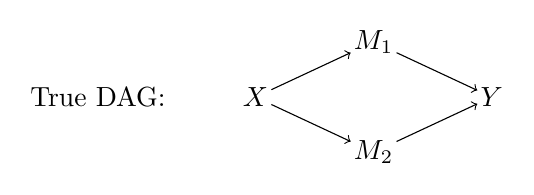
\begin{tikzpicture}[scale=1]
			\tikzstyle{every node}=[align=center, inner sep=1pt]
				\node (text) at (-2, 0) {True DAG:};
				\node (X) at (0, 0) {$ X $};
				\node (M1) at (1.5, 0.7) {$ M_1 $};
				\node (M2) at (1.5, -0.7) {$ M_2 $};
				\node (Y) at (3, 0) {$ Y $};
				\draw[->]  (X) -- (M1);
				\draw[->]  (X) -- (M2);
				\draw[->]  (M1) -- (Y);
				\draw[->]  (M2) -- (Y);
		\end{tikzpicture}
	\end{figure}

	\vspace{2em}
	\begin{figure}
	\centering
	\begin{tikzpicture}
		\begin{scope}
			\tikzstyle{every node}=[align=center, inner sep=1pt]
			\node (X) at (0, 0) {$ X $};
			\node (M1) at (1.5, 0.7) {$ M_1 $};
			\node (M2) at (1.5, -0.7) {$ M_2 $};
			\node (Y) at (3, 0) {$ Y $};

			\draw[dashed]  (X) -- (M1);
			\draw[dashed]  (X) -- (M2);
			\draw[dashed]  (M1) -- (Y);
			\draw[dashed]  (M2) -- (Y);
			\draw[dashed]  (X) -- (Y);
		\end{scope}
		\begin{scope}[xshift=3cm]
			\draw[->, ultra thick] (0.5, 0) -- (1, 0);
		\end{scope}
		\begin{scope}[xshift=4.5cm]
			\tikzstyle{every node}=[align=center, inner sep=1pt]
			\node (X) at (0, 0) {$ X $};
			\node (M1) at (1.5, 0.7) {$ M_1 $};
			\node (M2) at (1.5, -0.7) {$ M_2 $};
			\node (Y) at (3, 0) {$ Y $};

			\draw[dashed]  (X) -- (M1);
			\draw[dashed]  (X) -- (M2);
			\draw[dashed]  (M1) -- (Y);
			\draw[dashed]  (M2) -- (Y);
			\draw[->]  (X) -- (Y);
		\end{scope}
		\begin{scope}[xshift=7.5cm]
			\draw[->, ultra thick] (0.5, 0) -- (1, 0);
		\end{scope}
		\begin{scope}[xshift=9cm]
			\node at (0, 0) {$ \dots $};	
		\end{scope}
		\begin{scope}[xshift=9cm]
			\draw[->, ultra thick] (0, -0.5) -- (0, -1);
		\end{scope}
		\begin{scope}[xshift=7.5cm, yshift=-2.5cm]
			\tikzstyle{every node}=[align=center, inner sep=1pt]
			\node (X) at (0, 0) {$ X $};
			\node (M1) at (1.5, 0.7) {$ M_1 $};
			\node (M2) at (1.5, -0.7) {$ M_2 $};
			\node (Y) at (3, 0) {$ Y $};

			\draw[->]  (X) -- (M1);
			\draw[->]  (X) -- (M2);
			\draw[->]  (M1) -- (Y);
			\draw[->]  (M2) -- (Y);
			\draw[->, red]  (X) -- node[sloped, above] {\scriptsize $ 0 $} (Y);
		\end{scope}
		\begin{scope}[xshift=6.5cm, yshift=-2.5cm]
			\draw[->, ultra thick] (0.5, 0) -- (0, 0);
		\end{scope}
		\begin{scope}[xshift=3cm, yshift=-2.5cm]
			\tikzstyle{every node}=[align=center, inner sep=1pt]
			\node (X) at (0, 0) {$ X $};
			\node (M1) at (1.5, 0.7) {$ M_1 $};
			\node (M2) at (1.5, -0.7) {$ M_2 $};
			\node (Y) at (3, 0) {$ Y $};

			\draw[->]  (X) -- (M1);
			\draw[->]  (X) -- (M2);
			\draw[->]  (M1) -- (Y);
			\draw[->]  (M2) -- (Y);
		\end{scope}
		\begin{scope}[xshift=4.5cm, yshift=-4cm]
			\node at (0, 0) {Pruning};
		\end{scope}
	\end{tikzpicture}
	\caption*{Pruning Example}
	\end{figure}
\end{frame}

\begin{frame}{Empirical Analysis}
	\begin{figure}
		\centering
		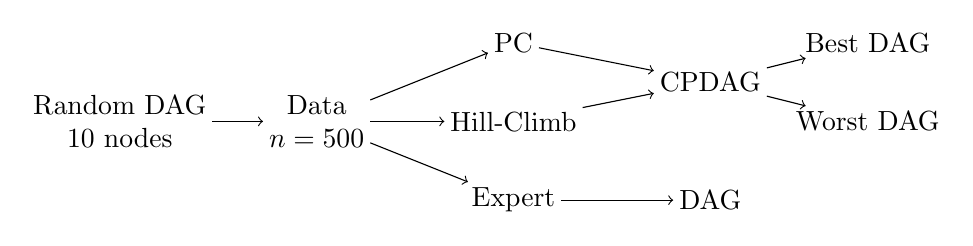
\begin{tikzpicture}
			\tikzstyle{every node}=[align=center, inner sep=2pt]
			\node (dag) at (0, 0) {Random DAG \\ $ 10 $ nodes};
			\node (data) at (2.5, 0) {Data \\ $ n=500 $};
			\node (pc) at (5, 1) {PC};
			\node (hc) at (5, 0) {Hill-Climb};
			\node (expert) at (5, -1) {Expert};
			\node (cpdag) at ( 7.5, 0.5) {CPDAG};
			\node (dag_l) at (7.5, -1) {DAG};
			\node (best_dag) at ( 9.5, 1 ) {Best DAG};
			\node (worst_dag) at ( 9.5, 0 ) {Worst DAG};

			\draw[->] (dag) -- (data);
			\draw[->] (data) -- (pc);
			\draw[->] (data) -- (hc);
			\draw[->] (data) -- (expert);
			\draw[->] (pc) -- (cpdag);
			\draw[->] (hc) -- (cpdag);
			\draw[->] (expert) -- (dag_l);
			\draw[->] (cpdag) -- (best_dag);
			\draw[->] (cpdag) -- (worst_dag);

		\end{tikzpicture}
	\end{figure}
	\vspace{2em}
	\begin{itemize}
		\item Linear mixed data is simulated.
		\item PC uses likelihood-ratio based MXM test.
		\item Hill-Climb Search uses BIC Score.
		\item The final DAGs are compared on Structural Hamming Distance (SHD) and Structural Intervention Distance (SID).
	\end{itemize}
\end{frame}


\begin{frame}{Empirical Analysis: Structural Hamming Distance}
	\begin{figure}
		\centering
		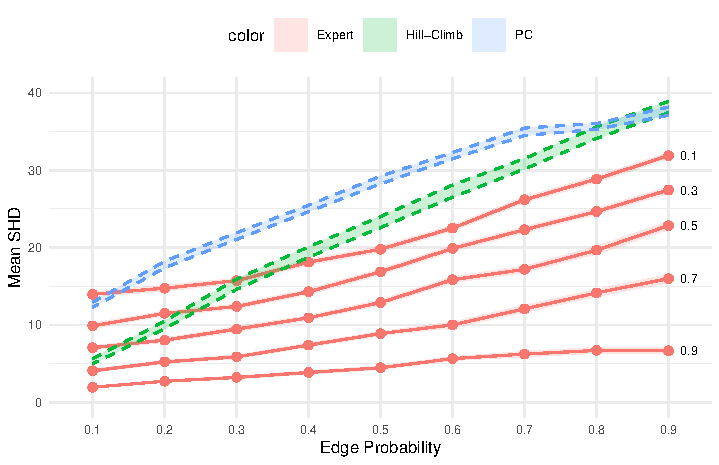
\includegraphics[scale=0.9]{../../2024-human-sl/code/plots/shd_ribbon.pdf}
		\caption{SHD vs edge probability}
	\end{figure}
\end{frame}

\begin{frame}{Empirical Analysis: Structural Intervention Distance}
	\begin{figure}
		\centering
		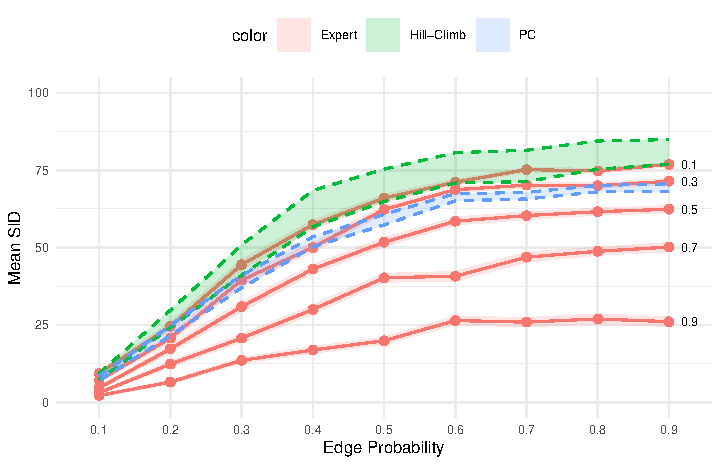
\includegraphics[scale=0.9]{../../2024-human-sl/code/plots/sid_ribbon.pdf}
		\caption{SID vs edge probability}
	\end{figure}
\end{frame}

\begin{frame}{LLMs as Oracles}
\end{frame}

\begin{frame}{Conclusion}
	\begin{itemize}
		\item We propose an effect size measure for mixed data.
		\item Using this effect size we built a web-based interactive tool to help researchers in creating DAGs from data.
		\item For oracles with reasonable accuracy we are able more accurate DAGs.
		\item The human simulator can get stuck in local minimas. Actual humans should perform better.
		\item Oracles can be replaced with LLMs.
	\end{itemize}
\end{frame}

\end{document}
